\section{Overview}
In order to understand \glspl{tee} we must first look at how computer architecture security worked before the problem of secure remote computation. The processor modes discussed in the introduction contained four \glspl{ring} with the most privileged level, \gls{ring} 0, executing operating system kernel code. However, in most modern x86 client systems there are 3 levels of even greater privilege than \gls{ring} 0. We will examine each of these briefly and describe why they do not provide the same type of protections that a \gls{tee} provides.

\section{The Predecessors of the TEE}

In 1990, Intel integrated a new privilege mode into their i386SL processor called \gls{smm} \cite{zimmer2005hardened}, now commonly referred to as ``\gls{ring} -2'' (\gls{ring} negative two).  OS code does not have access to this privilege level and only specific firmware, usually provided by the platform manufacturer, is allowed to execute code in \gls{smm}. This processor mode is entered by using a special \gls{smi}. This interrupt has the highest priority of any interrupt as of the writing of this thesis, and is even higher priority than a \gls{nmi}. Common tasks one might perform in \gls{smm} include thermal management, power management, or even something as simple as altering the volume output in response to buttons on a laptop keyboard \cite{yao2009system}. \gls{smm} would remain the most privileged level of code execution until the release of \gls{ime} in 2008 \cite{eldar2008configuring}.

The memory used in \gls{smm}, called \gls{smram}, is secured from any accesses or modifications originating anywhere outside \gls{smm}. Secured accesses include any accesses or modifications originating from the CPU, from I/O devices, and from \glspl{dma}. When an \gls{smi} is generated, all the CPU threads enter \gls{smm} and each of their register states are saved in a memory table inside \gls{smram}. Work can now be done by the \gls{smi} handler. Once this work is finished, each of the CPUs previous states are restored and execution is handed back to where the \gls{smi} was originally generated. Since there can be multiple \gls{smi} handlers there is firmware code that runs in a single thread and acts as an \gls{smi} dispatcher. All other CPU threads wait inside \gls{smm} until the handler thread has returned \cite{delgado2013}. This firmware code is an implementation of the \gls{uefi} specification, which is the successor to the \gls{efi} specification \cite{beyondBIOS}.

There are several reasons why \gls{smm} is not a suitable replacement for a \gls{tee}. Firstly, using \gls{smm} for any tasks which consume a significant amount of time would cause the system to hang while \glspl{smi} are handled. As such, \gls{smm} tasks are confined to small workloads which can return quickly and do not need to happen in rapid succession. However, tasks which take significant amounts of time and may occur in rapid succession are exactly the types of tasks we wish to run in a \gls{tee}. Tasks like processing a credit card payment, or verifying the identity of the user with biometrics would all take significant time to run and would need to happen in quick succession.

Secondly, \gls{smm} is very restrictive in terms of how code is developed for the platform. All code executed in \gls{smm} must be located inside the system firmware, loaded into \gls{smram}, and locked before the OS is loaded into memory. As such, firmware code does not have easy access to communicating with the host OS but must use special \gls{efi} \gls{smm} variables \cite{uefi2020}.

Lastly, while updating firmware in the field is possible \cite{zimmer2011apparatus}, it almost always requires a reboot of the system. Updating the code in a \gls{tee} is a critical function that will be required much more often than a firmware update and should not require system reboot each time. These are just a few reasons why \gls{smm} is not a suitable solution to the problem of secure remote computation. Perhaps the overarching reason is that \gls{smm} was not designed to solve the problem of secure remote computation. Regardless, we have shown why it should not be used where a \gls{tee} would be better suited.

In 2005 \cite{uhlig2005intel}, Intel released their first processor to allow the next most privileged mode of their x86 processors, \gls{vtx}\footnote{We use the acronym \gls{vtx} here to refer to all of Intel Virtualization Technologies, though in this case the ``x'' refers to Xeon processors with this feature. Non-Xeon processors would use the designation VT. There is also Intel Virtualization Technology for Directed I/O (VT-d). In this thesis we will use \gls{vtx} so as to avoid any confusion with the common acronym VT.}. Commonly referred to as ``\gls{ring} -1'' (ring negative one), \gls{vtx} added new instructions called \glspl{vms}. These instructions are used to create a layer of hardware isolation between the host OS from the guest OS. It is tempting to see a \gls{tee} as a type of virtualization. Indeed, one early form of a trusted computing environment used a ``dedicated closed virtual machine'' \cite{garfinkel2003terra} to achieve many of the goals of a modern \gls{tee}. However, as others have shown \cite{teeWhatIsIt}, this type of virtualization fails to cover several key properties of a \gls{tee}. For our purposes, we will consider these properties attestability and code confidentiality, and will discuss these in depth in coming chapters.

In 2008 \cite{eldar2008configuring}, Intel developed what is today the most privileged processor level on x86 hardware, the \glsreset{ime}\gls{ime}. This technology, commonly referred to as ``\gls{ring} -3'' (\gls{ring} negative three) is not actually a processor mode at all. It is instead a feature of some Intel chipsets. Most of the properties of \gls{ime} are obscured by the proprietary firmware that it runs. The majority of information available regarding \gls{ime} is found either in Intel's publications or from the plethora of reverse engineering done by security researchers. As such, we will not consider \gls{ime} a suitable replacement for a \gls{tee} for two key reasons: most of the information about this technology is gained by indirect means like reverse engineering and the firmware is not intended to be modified from the signed binary provided by Intel. 

These three x86 ``negative \glspl{ring}'' provide hardware protection of various kinds and each has its own restricted area of memory. However, none of these technologies serve as a viable solution to the problem of secure remote computation. It is no surprise that Intel eventually developed \gls{sgx}, their own implementation of a \gls{tee} in order to address this problem. Before we address \gls{sgx} specifically, we will continue to track the development of \glsreset{tee}\glspl{tee} by starting with their use in handsets, the precursor to today's smartphones.

\section{Birth of a TEE}

The concept of securing computation is not a new idea. As we have seen with \gls{ime}, neither is the technique of using a processor other than the main, general purpose CPU for secure computation. For almost two decades \cite{osborn2013trusted} hardware manufacturers have relied on \glspl{tpm} for a similar kind of secure computation. In 2009 the \gls{tcg} specification for a \gls{tpm} was ratified as an ISO standard. A \gls{tpm} is a system that must remain separate from the system it reports to: the host system. It can be a single physical component that communicates with the host system over a simple bus. \glspl{tpm} can have their own processor, RAM, ROM, and flash memory. While the host system cannot directly change the values of the \gls{tpm} memory, it can use the simple bus to send and receive information. As of \gls{tpm} version 2.0, the \gls{tpm} can now be a part of the main processor, however it must use hardware memory partitioning and use a well defined interface instead of the simple bus. The use of the main processor as a \gls{tpm} may add significantly more speed, but at the cost of more complexity. \glspl{tpm} contain random number generators, cryptography key generators, and secure storage.

While \glspl{tpm} have many of the features we require of our \glspl{tee}, they were designed with securing small amounts of data like cryptographic keys, not entire applications. \glspl{tpm} focus on security over speed and their cryptographic algorithms may be purposely run at much slower speeds than is possible with a CPU, let alone a cryptographic accelerator. \glspl{tpm} do, however, provide a valuable tool for a \gls{tee} to use as part of its \gls{chain of trust}\footnote{Unsurprisingly, the concept of a ``chain of trust'' comes out of electronic commerce security publications from the 1990's \cite{679731}. The internet opened up the concept of electronic commerce to a much broader audience. In doing so, it also opened up a much larger attack surface for threat models to consider.}. Concepts used in a \gls{tpm} like secure storage and isolated memory are expanded in a \gls{tee} with concepts like isolated and protected IO and isolated RAM. It is not surprising that we see the first industry efforts around \glspl{tee} around the same time that the ISO standard for \glspl{tpm} is published.

\glspl{tee} were first defined by the \gls{omtp} Hardware Working Group and ratified in 2009 \cite{Confidential2009}. This standard was designed specifically for ``handset manufacturers''. The \gls{omtp} standard was transferred to the Wholesale Applications Community (WAC) in 2010 and in July 2012 WAC itself was closed, with the \gls{omtp} standards being transferred to The GSM Association (originally Groupe Sp\'ecial Mobile) \cite{WAC}. The \gls{omtp} standard defines an ``execution environment'' as a combination of five elements: a processing unit, a bus, physical memory, a boot process, and the contents of the execution environment \cite{Confidential2009}. These contents include the code, data, and keys required for computation. The \gls{omtp} document goes on to describe two sets of security requirements which meet their definition of a \gls{tee}, called ``Profile 1 and 2''. Profile 2 provides greater security than Profile 1, however both meet their definition of a \gls{tee}.

\renewcommand{\arraystretch}{2}
\begin{table}[htb]
\centering
\begin{tabular}{|p{2cm}|p{12cm}|}
\hline
\textbf{Group} & \textbf{Attack Surface} \\ \hline
Group 1 & Hardware modules used for accessing memories, only including attacks mounted via modules built into the ``mobile equipment'' design (e.g. \gls{dma} module) \\ \hline
Group 2 & Colour LCD controllers or ``graphics chip of the mobile device'' designed to be pointed at memory blocks and could dump that information to the screen\\ \hline
Group 3 & Removal of battery or external memory card \\ \hline
Group 4 & Replacement of flash when power is off \\ \hline
Group 5 & Extract secrets by bus monitoring (e.g. hardware probes) \\ \hline
Group 6 & Attached devices (mod chips) used to attack data between flash and the \gls{soc} or in external RAM. \\ \hline
Group 7 & Replacement of flash when power is on \\ \hline
\end{tabular}
\caption[OMTP Threat Groups]{\textbf{Attack surfaces as grouped by the \gls{omtp}.} This table is created from data available in section 2.1 of the \gls{omtp} document. \cite{Confidential2009}}
\label{table:omtp_threat_groups}
\end{table}


Both profiles provide protection against unauthorized memory access given a list of vulnerable attack surfaces summarized in Table~\ref{table:omtp_threat_groups}. The core requirements for an \gls{omtp} \gls{tee} cover these ``threat groups'' to different degrees. There are 27 core requirements in total and it is out of the scope of this thesis to list or go into details on them. Sufficed to say that they address the attack surfaces described in Table~\ref{table:omtp_threat_groups}. Also, it is clear from the threat groups described that these threat models are only applicable to handsets and do not cover typical embedded devices. Another standards body called GlobalPlatform took up the task of standardizing the use of \glspl{tee} across multiple embedded platforms.

GlobalPlatform Incorporated is a nonprofit industry organization that began in 1999 with the mission of providing standardization around mobile payment devices and software. In 2011 they created a \gls{tee} model \cite{GlobalPlatform2018} that met the needs of embedded use cases. They define a \gls{tee} as a system providing ``isolated execution, integrity of \glspl{ta}, and integrity and confidentiality of \gls{ta} assets'' \cite{GlobalPlatform2018}. A GlobalPlatform \gls{tee} is more rigorous than the \gls{omtp} standard in that it requires a security certification provided by GlobalPlatform and must comply with the following GlobalPlatform standards: \gls{tee} Protection Profile, \gls{tee} Client API Specification, and \gls{tee} Internal Core API Specification \cite{GPD2, GPD3, GPD4}.

Unlike in the \gls{omtp} standard, GlobalPlatform first introduces the concept of \gls{attestation} in its definition of a \gls{rot}. We will discuss \gls{attestation} in depth for each of our technologies we cover, as well as in \autoref{chap:comp} where we consider this property of a TEE and if it can be considered optional \cite{cccTAC}. Standards and specifications from groups like \gls{omtp} and GlobalPlatforms paved the way for the creation of mobile devices capable of secure remote computation. Indeed, the smartphone revolution would only have been possible with the ability to run trusted applications allowing users to interact with financial, healthcare, and other valuable data.

\begin{figure}[htbp]
\centering
% Graphic for TeX using PGF
% Title: GPD-TEE.dia
% Creator: Dia v0.97.2
% CreationDate: Sun Feb 14 09:26:53 2021
% For: hume stephano
% \usepackage{tikz}
% The following commands are not supported in PSTricks at present
% We define them conditionally, so when they are implemented,
% this pgf file will use them.
\ifx\du\undefined
  \newlength{\du}
\fi
\setlength{\du}{15\unitlength}
\resizebox{.75\textwidth}{!}{%
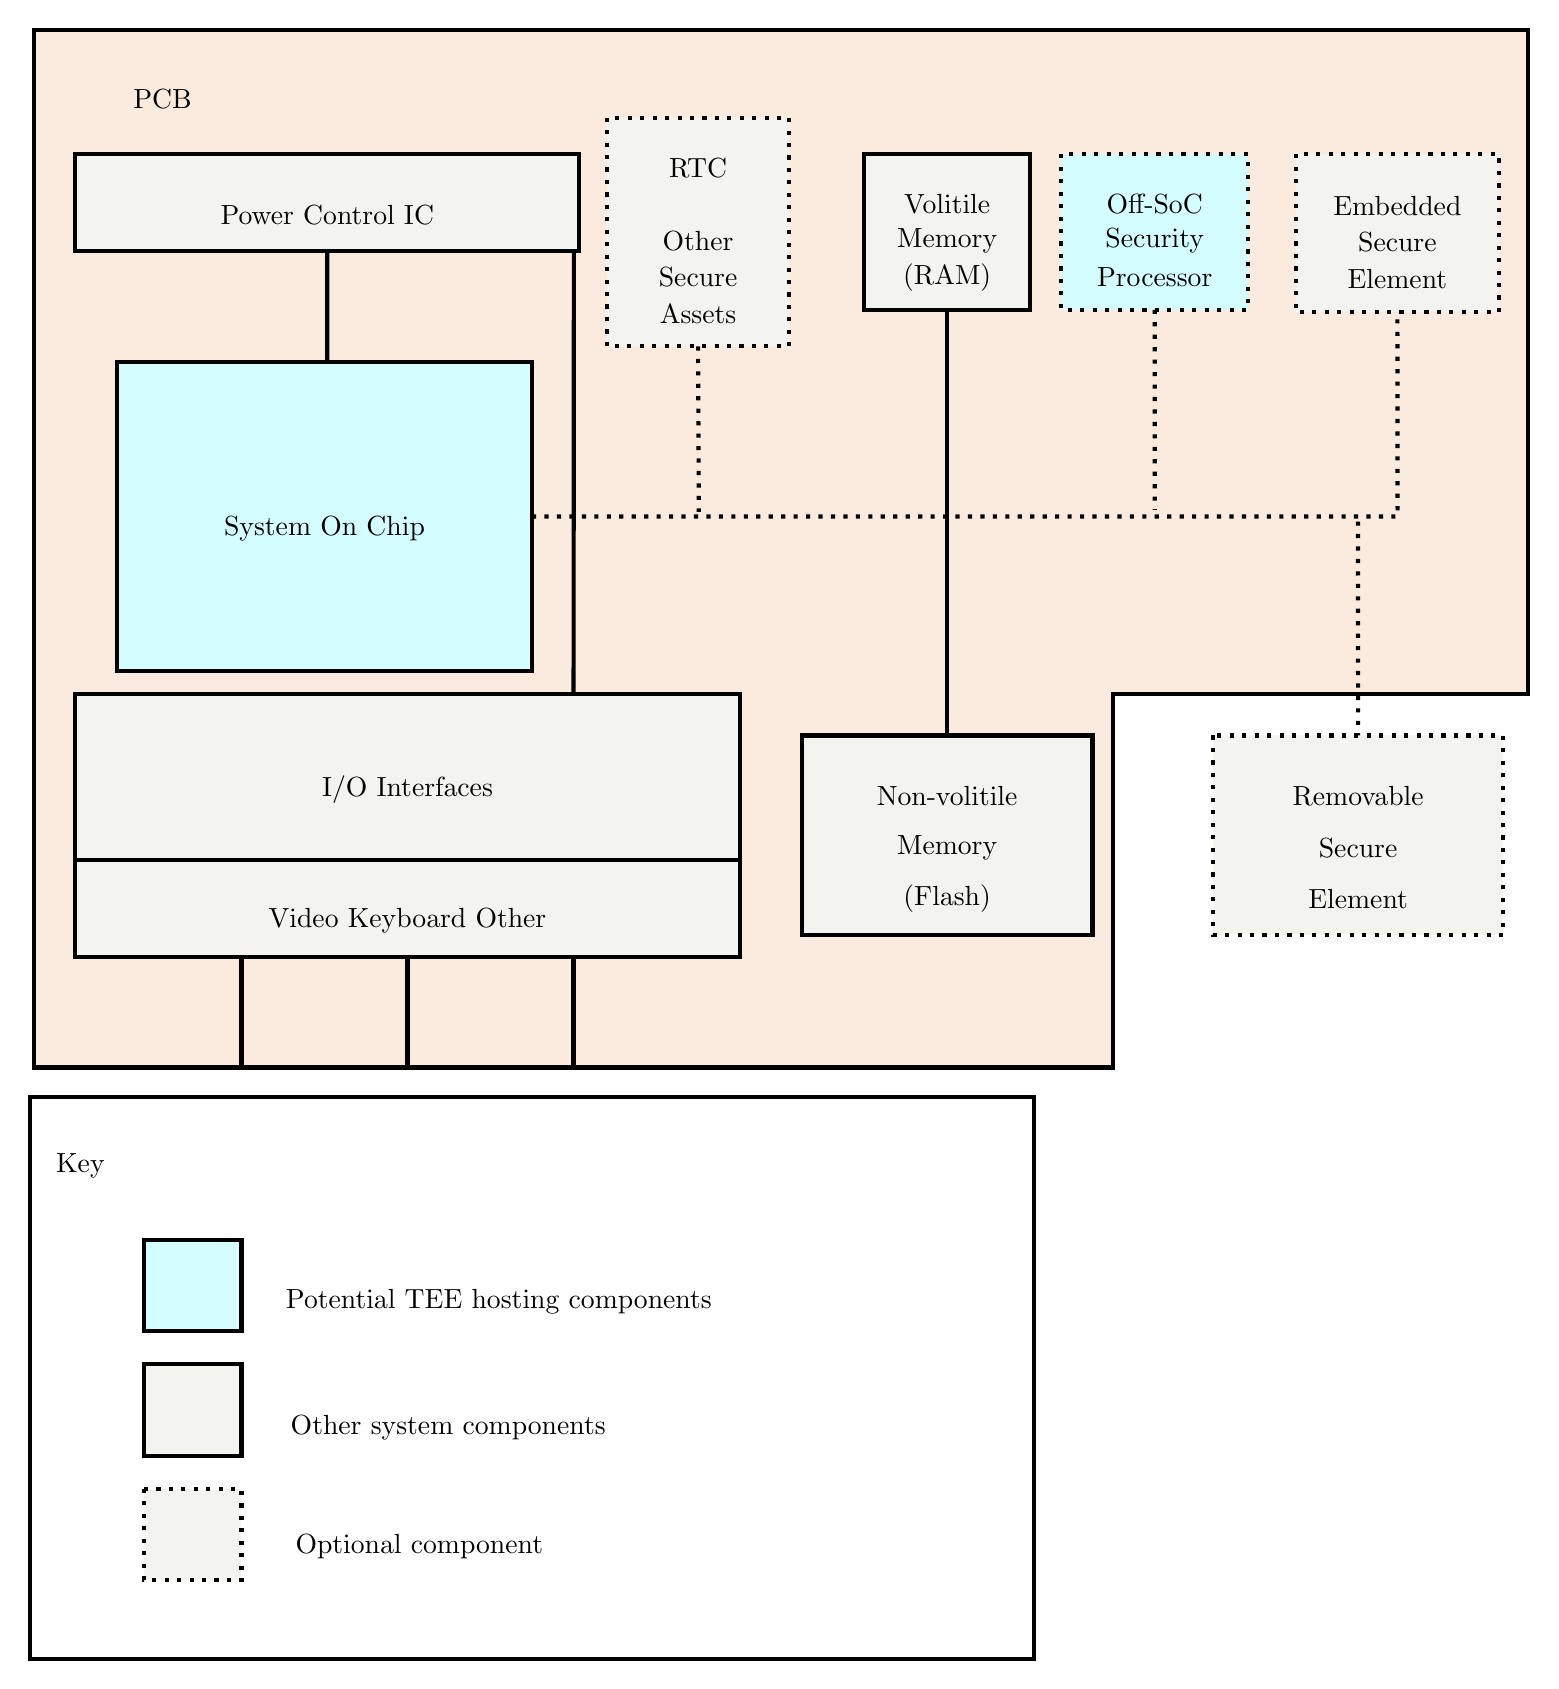
\begin{tikzpicture}
\pgftransformxscale{1.000000}
\pgftransformyscale{-1.000000}
\definecolor{dialinecolor}{rgb}{0.000000, 0.000000, 0.000000}
\pgfsetstrokecolor{dialinecolor}
\definecolor{dialinecolor}{rgb}{1.000000, 1.000000, 1.000000}
\pgfsetfillcolor{dialinecolor}
\pgfsetlinewidth{0.100000\du}
\pgfsetdash{}{0pt}
\pgfsetdash{}{0pt}
\pgfsetmiterjoin
\definecolor{dialinecolor}{rgb}{1.000000, 1.000000, 1.000000}
\pgfsetfillcolor{dialinecolor}
\fill (9.900000\du,30.700000\du)--(9.900000\du,44.250000\du)--(34.100000\du,44.250000\du)--(34.100000\du,30.700000\du)--cycle;
\definecolor{dialinecolor}{rgb}{0.000000, 0.000000, 0.000000}
\pgfsetstrokecolor{dialinecolor}
\draw (9.900000\du,30.700000\du)--(9.900000\du,44.250000\du)--(34.100000\du,44.250000\du)--(34.100000\du,30.700000\du)--cycle;
\pgfsetlinewidth{0.100000\du}
\pgfsetdash{}{0pt}
\pgfsetdash{}{0pt}
\pgfsetmiterjoin
\pgfsetbuttcap
\definecolor{dialinecolor}{rgb}{0.984314, 0.921569, 0.874510}
\pgfsetfillcolor{dialinecolor}
\fill (10.000000\du,5.000000\du)--(46.000000\du,5.000000\du)--(46.000000\du,21.000000\du)--(36.000000\du,21.000000\du)--(36.000000\du,30.000000\du)--(10.000000\du,30.000000\du)--cycle;
\definecolor{dialinecolor}{rgb}{0.000000, 0.000000, 0.000000}
\pgfsetstrokecolor{dialinecolor}
\draw (10.000000\du,5.000000\du)--(46.000000\du,5.000000\du)--(46.000000\du,21.000000\du)--(36.000000\du,21.000000\du)--(36.000000\du,30.000000\du)--(10.000000\du,30.000000\du)--cycle;
\pgfsetlinewidth{0.000000\du}
\pgfsetdash{}{0pt}
\pgfsetdash{}{0pt}
\pgfsetmiterjoin
\definecolor{dialinecolor}{rgb}{0.984314, 0.921569, 0.874510}
\pgfsetstrokecolor{dialinecolor}
\draw (10.100000\du,5.100000\du)--(10.100000\du,7.550000\du)--(16.100000\du,7.550000\du)--(16.100000\du,5.100000\du)--cycle;
% setfont left to latex
\definecolor{dialinecolor}{rgb}{0.000000, 0.000000, 0.000000}
\pgfsetstrokecolor{dialinecolor}
\node at (13.100000\du,6.669444\du){PCB};
\definecolor{dialinecolor}{rgb}{0.949020, 0.956863, 0.929412}
\pgfsetfillcolor{dialinecolor}
\fill (11.000000\du,8.000000\du)--(11.000000\du,10.334722\du)--(23.133750\du,10.334722\du)--(23.133750\du,8.000000\du)--cycle;
\pgfsetlinewidth{0.100000\du}
\pgfsetdash{}{0pt}
\pgfsetdash{}{0pt}
\pgfsetmiterjoin
\definecolor{dialinecolor}{rgb}{0.000000, 0.000000, 0.000000}
\pgfsetstrokecolor{dialinecolor}
\draw (11.000000\du,8.000000\du)--(11.000000\du,10.334722\du)--(23.133750\du,10.334722\du)--(23.133750\du,8.000000\du)--cycle;
% setfont left to latex
\definecolor{dialinecolor}{rgb}{0.000000, 0.000000, 0.000000}
\pgfsetstrokecolor{dialinecolor}
\node at (17.066875\du,9.467500\du){Power Control IC};
\definecolor{dialinecolor}{rgb}{0.827451, 0.992157, 0.996078}
\pgfsetfillcolor{dialinecolor}
\fill (12.000000\du,13.000000\du)--(12.000000\du,20.450000\du)--(22.000000\du,20.450000\du)--(22.000000\du,13.000000\du)--cycle;
\pgfsetlinewidth{0.100000\du}
\pgfsetdash{}{0pt}
\pgfsetdash{}{0pt}
\pgfsetmiterjoin
\definecolor{dialinecolor}{rgb}{0.000000, 0.000000, 0.000000}
\pgfsetstrokecolor{dialinecolor}
\draw (12.000000\du,13.000000\du)--(12.000000\du,20.450000\du)--(22.000000\du,20.450000\du)--(22.000000\du,13.000000\du)--cycle;
% setfont left to latex
\definecolor{dialinecolor}{rgb}{0.000000, 0.000000, 0.000000}
\pgfsetstrokecolor{dialinecolor}
\node at (17.000000\du,17.025139\du){System On Chip};
\definecolor{dialinecolor}{rgb}{0.949020, 0.956863, 0.929412}
\pgfsetfillcolor{dialinecolor}
\fill (11.000000\du,21.000000\du)--(11.000000\du,25.000000\du)--(27.000000\du,25.000000\du)--(27.000000\du,21.000000\du)--cycle;
\pgfsetlinewidth{0.100000\du}
\pgfsetdash{}{0pt}
\pgfsetdash{}{0pt}
\pgfsetmiterjoin
\definecolor{dialinecolor}{rgb}{0.000000, 0.000000, 0.000000}
\pgfsetstrokecolor{dialinecolor}
\draw (11.000000\du,21.000000\du)--(11.000000\du,25.000000\du)--(27.000000\du,25.000000\du)--(27.000000\du,21.000000\du)--cycle;
% setfont left to latex
\definecolor{dialinecolor}{rgb}{0.000000, 0.000000, 0.000000}
\pgfsetstrokecolor{dialinecolor}
\node at (19.000000\du,23.300139\du){I/O Interfaces};
\definecolor{dialinecolor}{rgb}{0.949020, 0.956863, 0.929412}
\pgfsetfillcolor{dialinecolor}
\fill (11.000000\du,25.000000\du)--(11.000000\du,27.334722\du)--(27.000000\du,27.334722\du)--(27.000000\du,25.000000\du)--cycle;
\pgfsetlinewidth{0.100000\du}
\pgfsetdash{}{0pt}
\pgfsetdash{}{0pt}
\pgfsetmiterjoin
\definecolor{dialinecolor}{rgb}{0.000000, 0.000000, 0.000000}
\pgfsetstrokecolor{dialinecolor}
\draw (11.000000\du,25.000000\du)--(11.000000\du,27.334722\du)--(27.000000\du,27.334722\du)--(27.000000\du,25.000000\du)--cycle;
% setfont left to latex
\definecolor{dialinecolor}{rgb}{0.000000, 0.000000, 0.000000}
\pgfsetstrokecolor{dialinecolor}
\node at (19.000000\du,26.467500\du){Video  Keyboard  Other};
\definecolor{dialinecolor}{rgb}{0.949020, 0.956863, 0.929412}
\pgfsetfillcolor{dialinecolor}
\fill (28.500000\du,22.000000\du)--(28.500000\du,26.804167\du)--(35.500000\du,26.804167\du)--(35.500000\du,22.000000\du)--cycle;
\pgfsetlinewidth{0.100000\du}
\pgfsetdash{}{0pt}
\pgfsetdash{}{0pt}
\pgfsetmiterjoin
\definecolor{dialinecolor}{rgb}{0.000000, 0.000000, 0.000000}
\pgfsetstrokecolor{dialinecolor}
\draw (28.500000\du,22.000000\du)--(28.500000\du,26.804167\du)--(35.500000\du,26.804167\du)--(35.500000\du,22.000000\du)--cycle;
% setfont left to latex
\definecolor{dialinecolor}{rgb}{0.000000, 0.000000, 0.000000}
\pgfsetstrokecolor{dialinecolor}
\node at (32.000000\du,23.467500\du){Non-volitile};
% setfont left to latex
\definecolor{dialinecolor}{rgb}{0.000000, 0.000000, 0.000000}
\pgfsetstrokecolor{dialinecolor}
\node at (32.000000\du,24.702222\du){Memory};
% setfont left to latex
\definecolor{dialinecolor}{rgb}{0.000000, 0.000000, 0.000000}
\pgfsetstrokecolor{dialinecolor}
\node at (32.000000\du,25.936944\du){(Flash)};
\definecolor{dialinecolor}{rgb}{0.949020, 0.956863, 0.929412}
\pgfsetfillcolor{dialinecolor}
\fill (30.000000\du,8.000000\du)--(30.000000\du,11.745833\du)--(34.000000\du,11.745833\du)--(34.000000\du,8.000000\du)--cycle;
\pgfsetlinewidth{0.100000\du}
\pgfsetdash{}{0pt}
\pgfsetdash{}{0pt}
\pgfsetmiterjoin
\definecolor{dialinecolor}{rgb}{0.000000, 0.000000, 0.000000}
\pgfsetstrokecolor{dialinecolor}
\draw (30.000000\du,8.000000\du)--(30.000000\du,11.745833\du)--(34.000000\du,11.745833\du)--(34.000000\du,8.000000\du)--cycle;
% setfont left to latex
\definecolor{dialinecolor}{rgb}{0.000000, 0.000000, 0.000000}
\pgfsetstrokecolor{dialinecolor}
\node at (32.000000\du,9.205000\du){Volitile};
% setfont left to latex
\definecolor{dialinecolor}{rgb}{0.000000, 0.000000, 0.000000}
\pgfsetstrokecolor{dialinecolor}
\node at (32.000000\du,10.086944\du){Memory};
% setfont left to latex
\definecolor{dialinecolor}{rgb}{0.000000, 0.000000, 0.000000}
\pgfsetstrokecolor{dialinecolor}
\node at (32.000000\du,10.968889\du){(RAM)};
\definecolor{dialinecolor}{rgb}{0.949020, 0.956863, 0.929412}
\pgfsetfillcolor{dialinecolor}
\fill (40.400000\du,8.000000\du)--(40.400000\du,11.804167\du)--(45.292500\du,11.804167\du)--(45.292500\du,8.000000\du)--cycle;
\pgfsetlinewidth{0.100000\du}
\pgfsetdash{{\pgflinewidth}{0.200000\du}}{0cm}
\pgfsetdash{{\pgflinewidth}{0.200000\du}}{0cm}
\pgfsetmiterjoin
\definecolor{dialinecolor}{rgb}{0.000000, 0.000000, 0.000000}
\pgfsetstrokecolor{dialinecolor}
\draw (40.400000\du,8.000000\du)--(40.400000\du,11.804167\du)--(45.292500\du,11.804167\du)--(45.292500\du,8.000000\du)--cycle;
% setfont left to latex
\definecolor{dialinecolor}{rgb}{0.000000, 0.000000, 0.000000}
\pgfsetstrokecolor{dialinecolor}
\node at (42.846250\du,9.234167\du){Embedded};
% setfont left to latex
\definecolor{dialinecolor}{rgb}{0.000000, 0.000000, 0.000000}
\pgfsetstrokecolor{dialinecolor}
\node at (42.846250\du,10.116111\du){Secure};
% setfont left to latex
\definecolor{dialinecolor}{rgb}{0.000000, 0.000000, 0.000000}
\pgfsetstrokecolor{dialinecolor}
\node at (42.846250\du,10.998055\du){Element};
\definecolor{dialinecolor}{rgb}{0.949020, 0.956863, 0.929412}
\pgfsetfillcolor{dialinecolor}
\fill (38.400000\du,22.000000\du)--(38.400000\du,26.804167\du)--(45.400000\du,26.804167\du)--(45.400000\du,22.000000\du)--cycle;
\pgfsetlinewidth{0.100000\du}
\pgfsetdash{{\pgflinewidth}{0.200000\du}}{0cm}
\pgfsetdash{{\pgflinewidth}{0.200000\du}}{0cm}
\pgfsetmiterjoin
\definecolor{dialinecolor}{rgb}{0.000000, 0.000000, 0.000000}
\pgfsetstrokecolor{dialinecolor}
\draw (38.400000\du,22.000000\du)--(38.400000\du,26.804167\du)--(45.400000\du,26.804167\du)--(45.400000\du,22.000000\du)--cycle;
% setfont left to latex
\definecolor{dialinecolor}{rgb}{0.000000, 0.000000, 0.000000}
\pgfsetstrokecolor{dialinecolor}
\node at (41.900000\du,23.467500\du){Removable};
% setfont left to latex
\definecolor{dialinecolor}{rgb}{0.000000, 0.000000, 0.000000}
\pgfsetstrokecolor{dialinecolor}
\node at (41.900000\du,24.702222\du){Secure};
% setfont left to latex
\definecolor{dialinecolor}{rgb}{0.000000, 0.000000, 0.000000}
\pgfsetstrokecolor{dialinecolor}
\node at (41.900000\du,25.936944\du){Element};
\definecolor{dialinecolor}{rgb}{0.827451, 0.992157, 0.996078}
\pgfsetfillcolor{dialinecolor}
\fill (34.750000\du,8.000000\du)--(34.750000\du,11.745833\du)--(39.250000\du,11.745833\du)--(39.250000\du,8.000000\du)--cycle;
\pgfsetlinewidth{0.100000\du}
\pgfsetdash{{\pgflinewidth}{0.200000\du}}{0cm}
\pgfsetdash{{\pgflinewidth}{0.200000\du}}{0cm}
\pgfsetmiterjoin
\definecolor{dialinecolor}{rgb}{0.000000, 0.000000, 0.000000}
\pgfsetstrokecolor{dialinecolor}
\draw (34.750000\du,8.000000\du)--(34.750000\du,11.745833\du)--(39.250000\du,11.745833\du)--(39.250000\du,8.000000\du)--cycle;
% setfont left to latex
\definecolor{dialinecolor}{rgb}{0.000000, 0.000000, 0.000000}
\pgfsetstrokecolor{dialinecolor}
\node at (37.000000\du,9.205000\du){Off-SoC};
% setfont left to latex
\definecolor{dialinecolor}{rgb}{0.000000, 0.000000, 0.000000}
\pgfsetstrokecolor{dialinecolor}
\node at (37.000000\du,10.086944\du){Security};
% setfont left to latex
\definecolor{dialinecolor}{rgb}{0.000000, 0.000000, 0.000000}
\pgfsetstrokecolor{dialinecolor}
\node at (37.000000\du,10.968889\du){Processor};
\definecolor{dialinecolor}{rgb}{0.949020, 0.956863, 0.929412}
\pgfsetfillcolor{dialinecolor}
\fill (23.805000\du,7.118060\du)--(23.805000\du,12.627782\du)--(28.195000\du,12.627782\du)--(28.195000\du,7.118060\du)--cycle;
\pgfsetlinewidth{0.100000\du}
\pgfsetdash{{\pgflinewidth}{0.200000\du}}{0cm}
\pgfsetdash{{\pgflinewidth}{0.200000\du}}{0cm}
\pgfsetmiterjoin
\definecolor{dialinecolor}{rgb}{0.000000, 0.000000, 0.000000}
\pgfsetstrokecolor{dialinecolor}
\draw (23.805000\du,7.118060\du)--(23.805000\du,12.627782\du)--(28.195000\du,12.627782\du)--(28.195000\du,7.118060\du)--cycle;
% setfont left to latex
\definecolor{dialinecolor}{rgb}{0.000000, 0.000000, 0.000000}
\pgfsetstrokecolor{dialinecolor}
\node at (26.000000\du,8.323060\du){RTC};
% setfont left to latex
\definecolor{dialinecolor}{rgb}{0.000000, 0.000000, 0.000000}
\pgfsetstrokecolor{dialinecolor}
\node at (26.000000\du,9.205004\du){};
% setfont left to latex
\definecolor{dialinecolor}{rgb}{0.000000, 0.000000, 0.000000}
\pgfsetstrokecolor{dialinecolor}
\node at (26.000000\du,10.086949\du){Other};
% setfont left to latex
\definecolor{dialinecolor}{rgb}{0.000000, 0.000000, 0.000000}
\pgfsetstrokecolor{dialinecolor}
\node at (26.000000\du,10.968893\du){Secure};
% setfont left to latex
\definecolor{dialinecolor}{rgb}{0.000000, 0.000000, 0.000000}
\pgfsetstrokecolor{dialinecolor}
\node at (26.000000\du,11.850838\du){Assets};
\pgfsetlinewidth{0.100000\du}
\pgfsetdash{}{0pt}
\pgfsetdash{}{0pt}
\pgfsetbuttcap
{
\definecolor{dialinecolor}{rgb}{0.000000, 0.000000, 0.000000}
\pgfsetfillcolor{dialinecolor}
% was here!!!
\definecolor{dialinecolor}{rgb}{0.000000, 0.000000, 0.000000}
\pgfsetstrokecolor{dialinecolor}
\draw (17.066900\du,10.334700\du)--(17.067965\du,12.962354\du);
}
\pgfsetlinewidth{0.100000\du}
\pgfsetdash{}{0pt}
\pgfsetdash{}{0pt}
\pgfsetbuttcap
{
\definecolor{dialinecolor}{rgb}{0.000000, 0.000000, 0.000000}
\pgfsetfillcolor{dialinecolor}
% was here!!!
\definecolor{dialinecolor}{rgb}{0.000000, 0.000000, 0.000000}
\pgfsetstrokecolor{dialinecolor}
\draw (23.007662\du,10.346059\du)--(23.000000\du,21.000000\du);
}
\pgfsetlinewidth{0.100000\du}
\pgfsetdash{}{0pt}
\pgfsetdash{}{0pt}
\pgfsetbuttcap
{
\definecolor{dialinecolor}{rgb}{0.000000, 0.000000, 0.000000}
\pgfsetfillcolor{dialinecolor}
% was here!!!
\definecolor{dialinecolor}{rgb}{0.000000, 0.000000, 0.000000}
\pgfsetstrokecolor{dialinecolor}
\draw (23.000000\du,27.334700\du)--(23.000000\du,30.000000\du);
}
\pgfsetlinewidth{0.100000\du}
\pgfsetdash{}{0pt}
\pgfsetdash{}{0pt}
\pgfsetbuttcap
{
\definecolor{dialinecolor}{rgb}{0.000000, 0.000000, 0.000000}
\pgfsetfillcolor{dialinecolor}
% was here!!!
\definecolor{dialinecolor}{rgb}{0.000000, 0.000000, 0.000000}
\pgfsetstrokecolor{dialinecolor}
\draw (19.000000\du,27.334700\du)--(19.000000\du,30.000000\du);
}
\pgfsetlinewidth{0.100000\du}
\pgfsetdash{}{0pt}
\pgfsetdash{}{0pt}
\pgfsetbuttcap
{
\definecolor{dialinecolor}{rgb}{0.000000, 0.000000, 0.000000}
\pgfsetfillcolor{dialinecolor}
% was here!!!
\definecolor{dialinecolor}{rgb}{0.000000, 0.000000, 0.000000}
\pgfsetstrokecolor{dialinecolor}
\draw (15.000000\du,27.334700\du)--(15.000000\du,30.000000\du);
}
\pgfsetlinewidth{0.100000\du}
\pgfsetdash{}{0pt}
\pgfsetdash{}{0pt}
\pgfsetbuttcap
{
\definecolor{dialinecolor}{rgb}{0.000000, 0.000000, 0.000000}
\pgfsetfillcolor{dialinecolor}
% was here!!!
\definecolor{dialinecolor}{rgb}{0.000000, 0.000000, 0.000000}
\pgfsetstrokecolor{dialinecolor}
\draw (32.000000\du,11.745800\du)--(32.000000\du,17.000000\du);
}
\pgfsetlinewidth{0.100000\du}
\pgfsetdash{}{0pt}
\pgfsetdash{}{0pt}
\pgfsetbuttcap
{
\definecolor{dialinecolor}{rgb}{0.000000, 0.000000, 0.000000}
\pgfsetfillcolor{dialinecolor}
% was here!!!
\definecolor{dialinecolor}{rgb}{0.000000, 0.000000, 0.000000}
\pgfsetstrokecolor{dialinecolor}
\draw (32.000000\du,17.000000\du)--(32.000000\du,21.950685\du);
}
\pgfsetlinewidth{0.100000\du}
\pgfsetdash{}{0pt}
\pgfsetdash{}{0pt}
\pgfsetmiterjoin
\definecolor{dialinecolor}{rgb}{0.827451, 0.992157, 0.996078}
\pgfsetfillcolor{dialinecolor}
\fill (12.650000\du,34.150000\du)--(12.650000\du,36.350000\du)--(15.000000\du,36.350000\du)--(15.000000\du,34.150000\du)--cycle;
\definecolor{dialinecolor}{rgb}{0.000000, 0.000000, 0.000000}
\pgfsetstrokecolor{dialinecolor}
\draw (12.650000\du,34.150000\du)--(12.650000\du,36.350000\du)--(15.000000\du,36.350000\du)--(15.000000\du,34.150000\du)--cycle;
% setfont left to latex
\definecolor{dialinecolor}{rgb}{0.000000, 0.000000, 0.000000}
\pgfsetstrokecolor{dialinecolor}
\node[anchor=west] at (15.800000\du,35.650000\du){Potential TEE hosting components};
\pgfsetlinewidth{0.100000\du}
\pgfsetdash{}{0pt}
\pgfsetdash{}{0pt}
\pgfsetmiterjoin
\definecolor{dialinecolor}{rgb}{0.949020, 0.956863, 0.929412}
\pgfsetfillcolor{dialinecolor}
\fill (12.650000\du,37.150000\du)--(12.650000\du,39.350000\du)--(15.000000\du,39.350000\du)--(15.000000\du,37.150000\du)--cycle;
\definecolor{dialinecolor}{rgb}{0.000000, 0.000000, 0.000000}
\pgfsetstrokecolor{dialinecolor}
\draw (12.650000\du,37.150000\du)--(12.650000\du,39.350000\du)--(15.000000\du,39.350000\du)--(15.000000\du,37.150000\du)--cycle;
% setfont left to latex
\definecolor{dialinecolor}{rgb}{0.000000, 0.000000, 0.000000}
\pgfsetstrokecolor{dialinecolor}
\node[anchor=west] at (15.915000\du,38.670000\du){Other system components};
\pgfsetlinewidth{0.100000\du}
\pgfsetdash{{\pgflinewidth}{0.200000\du}}{0cm}
\pgfsetdash{{\pgflinewidth}{0.200000\du}}{0cm}
\pgfsetmiterjoin
\definecolor{dialinecolor}{rgb}{0.949020, 0.956863, 0.929412}
\pgfsetfillcolor{dialinecolor}
\fill (12.650000\du,40.150000\du)--(12.650000\du,42.350000\du)--(15.000000\du,42.350000\du)--(15.000000\du,40.150000\du)--cycle;
\definecolor{dialinecolor}{rgb}{0.000000, 0.000000, 0.000000}
\pgfsetstrokecolor{dialinecolor}
\draw (12.650000\du,40.150000\du)--(12.650000\du,42.350000\du)--(15.000000\du,42.350000\du)--(15.000000\du,40.150000\du)--cycle;
% setfont left to latex
\definecolor{dialinecolor}{rgb}{0.000000, 0.000000, 0.000000}
\pgfsetstrokecolor{dialinecolor}
\node[anchor=west] at (16.030000\du,41.540000\du){Optional component};
% setfont left to latex
\definecolor{dialinecolor}{rgb}{0.000000, 0.000000, 0.000000}
\pgfsetstrokecolor{dialinecolor}
\node[anchor=west] at (10.265000\du,32.362500\du){Key};
\pgfsetlinewidth{0.100000\du}
\pgfsetdash{{\pgflinewidth}{0.200000\du}}{0cm}
\pgfsetdash{{\pgflinewidth}{0.200000\du}}{0cm}
\pgfsetmiterjoin
\pgfsetbuttcap
{
\definecolor{dialinecolor}{rgb}{0.000000, 0.000000, 0.000000}
\pgfsetfillcolor{dialinecolor}
% was here!!!
{\pgfsetcornersarced{\pgfpoint{0.000000\du}{0.000000\du}}\definecolor{dialinecolor}{rgb}{0.000000, 0.000000, 0.000000}
\pgfsetstrokecolor{dialinecolor}
\draw (22.000000\du,16.725000\du)--(42.850542\du,16.725201\du)--(42.846250\du,11.804167\du);
}}
\pgfsetlinewidth{0.100000\du}
\pgfsetdash{{\pgflinewidth}{0.200000\du}}{0cm}
\pgfsetdash{{\pgflinewidth}{0.200000\du}}{0cm}
\pgfsetbuttcap
{
\definecolor{dialinecolor}{rgb}{0.000000, 0.000000, 0.000000}
\pgfsetfillcolor{dialinecolor}
% was here!!!
\definecolor{dialinecolor}{rgb}{0.000000, 0.000000, 0.000000}
\pgfsetstrokecolor{dialinecolor}
\draw (41.895948\du,16.846873\du)--(41.900000\du,22.000000\du);
}
\pgfsetlinewidth{0.100000\du}
\pgfsetdash{{\pgflinewidth}{0.200000\du}}{0cm}
\pgfsetdash{{\pgflinewidth}{0.200000\du}}{0cm}
\pgfsetbuttcap
{
\definecolor{dialinecolor}{rgb}{0.000000, 0.000000, 0.000000}
\pgfsetfillcolor{dialinecolor}
% was here!!!
\definecolor{dialinecolor}{rgb}{0.000000, 0.000000, 0.000000}
\pgfsetstrokecolor{dialinecolor}
\draw (37.000000\du,11.745833\du)--(36.999117\du,16.564188\du);
}
\pgfsetlinewidth{0.100000\du}
\pgfsetdash{{\pgflinewidth}{0.200000\du}}{0cm}
\pgfsetdash{{\pgflinewidth}{0.200000\du}}{0cm}
\pgfsetbuttcap
{
\definecolor{dialinecolor}{rgb}{0.000000, 0.000000, 0.000000}
\pgfsetfillcolor{dialinecolor}
% was here!!!
\definecolor{dialinecolor}{rgb}{0.000000, 0.000000, 0.000000}
\pgfsetstrokecolor{dialinecolor}
\draw (26.000000\du,12.627782\du)--(26.017331\du,16.614188\du);
}
\end{tikzpicture}
}


\caption[GlobalPlatforms Typical Chipset Architecture]{\textbf{The board level chipset architecture of a typical mobile device.} The concept of an embedded or removable secure element allows for devices like a \gls{tpm} which may hold secure data but will not host the \gls{tee}. A \gls{tee} may reside on the SoC itself as with Arm TrustZone. However, it is possible to physically separate the \gls{tee} from the SoC and still be compliant with the GlobalPlatform model. This figure was recreated and simplified from Figure 2-1 on page 15 of the GlobalPlatform Technology TEE System Architecture Version 1.2. \cite{GlobalPlatform2018}.}
\label{fig:gpd-tee}
\end{figure}

In Figure~\ref{fig:gpd-tee} we see a very common mobile device system diagram with the possible \gls{tee} hosting components listed as both on and off chip. GlobalPlatforms differentiates between the \gls{ree} and the \glsreset{tee}\gls{tee}. The \gls{ree} focuses on extensibility and versatility whereas the \gls{tee} has only one purpose: to ``provide a safe area of the device to protect assets and execute trusted code'' \cite{GlobalPlatform2018}.  These standards were first put into use by complex \glspl{soc} with the release of processors implementing the ARM Cortex A5 core in 2012. These cores included Arm TrustZone as well as a reference firmware implementation for building secure applications. Arm TrustZone has since become the de facto standard for embedded devices as well as as Android-based mobile phones requiring a \gls{tee}. 

Up to now, we have only covered relatively simple use cases like handsets, smartphones, and embedded devices. Bridging the gap between these simple devices and desktop or server processors will require we cover the current dominant architecture in that space, namely the x86 family implemented by Intel and AMD.

\section{From Handsets to the Cloud}
In 2013 at a workshop titled Hardware and Architectural Support for Security and Privacy (HASP), Intel introduced \glsreset{sgx}\gls{sgx} for Intel architecture. \gls{sgx} is not an extension to the x86 architecture, but rather to the Intel architecture. As such, AMD developed their own solution called \gls{sev}. As mentioned previously, we will not discuss AMD \gls{sev} in this thesis as its architecture is quite different from Intel \gls{sgx}. While there are several papers published in the proceedings from the HASP 2013 workshop \cite{10.1145/2487726.2488368, 10.1145/2487726.2488370, anati2013innovative}, as well as two patents from Intel's original filings \cite{johnson2010technique, mckeen2009method}, we will use a more recent paper by Costan \cite{Costan2016} as well as a recent whitepaper from Intel \cite{johnson2016intel} in exploring \gls{sgx}.

Intel's introduction of \gls{sgx} opened up the desktop and laptop markets to a new type of software application capable of hardware-backed secure ``enclaves''. It also gave application developers on Intel platforms the chance to utilize both local and remote \gls{attestation}, providing assurance from the vendor regarding code integrity and confidentiality. It wasn't until 2021 that Intel would make this technology available in multi-socket Xeon CPUs, opening the door for cloud providers to take advantage of \glspl{tee} on Intel platforms \cite{10.1145/3337167.3337173}.

\section{RISC-V: An Open Source TEE}
RISC-V is a popular modern architecture developed at the Parallel Computing Lab (Par Lab), which is part of the University of California at Berkeley. Perhaps the most notable thing about this architecture is that it has been developed using the same methodology as open source software. The specifications are published using a Creative Commons license, and all code examples or artifacts of the specification use permissive licenses like the BSD licenses or the Apache license \cite{UnprivIsa2019}. The work done on the RISC-V specifications is overseen by a non-profit organization called RISC-V International, an organization registered in Switzerland.

The Trusted Execution Environment Task Group of RISC-V International has developed a specification called \gls{pmp} as part of the RISC-V Privileged Specification \cite{PrivIsa2019}. RISC-V \gls{pmp} extends the concept of \gls{pma} to include multiple configurable sections of memory whose access rights can be altered by firmware running at the highest privilege level. RISC-V \gls{pmp} is certainly a very basic type of \gls{tee}, however plans to extend its capabilities have already been drafted in a new specification called \gls{epmp}. Likewise, drafts of \gls{spmp} and \gls{iopmp} are set for ratification in 2021. We will discuss all of these types of memory protection in detail in \autoref{chap:pmp}.

This chapter has given a brief background of \glsreset{tee}\glspl{tee} and we have been selective in mentioning only a few of the many examples of hardware security that influenced the development of \glspl{tee}. We have shown that any given \gls{tee} builds off the technologies of the past, even when incorporating new instructions or hardware unique to \glspl{tee}. As we will see, without technologies and standards like the \gls{tpm} ISO standard of 2009, \glspl{tee} would not have the means to perform many of the advanced features like attestation which are critical to some applications. We continue now with an overview of our three technologies for comparison: Intel \glsreset{sgx}\gls{sgx}, Arm TrustZone, and RISC-V \glsreset{pmp}\gls{pmp}.

\begin{table}
\renewcommand\arraystretch{2}
\begin{tabular}{@{\,}r <{\hskip 2pt} !{\foo} >{\raggedright\arraybackslash}p{10cm}}
\toprule
\addlinespace[1.5ex]
1990 & Intel releases \gls{smm} \\
2005 & First processor using \gls{vtx} released \\
2006 & \textcolor{red}{Firmware vulnerabilities in \gls{smm} found} \\
2008 & \gls{ime} released \linebreak \textcolor{red}{First VM Escape CVEs found} \\
2009 & \textcolor{blue}{\gls{omtp} \glspl{tee} spec and \gls{tpm} ISO standard} \\
2011 & \textcolor{blue}{GlobalPlatform \gls{tee} spec} \\
2012 & \textcolor{blue}{ARM Cortex-A5 with TrustZone} \\
2013 & \textcolor{red}{TrustZone vulnerability found} \linebreak \textcolor{blue}{Intel introduces \glsreset{sgx}\gls{sgx}} \\
2015 & \textcolor{blue}{Intel Skylake with \gls{sgx}} \\
2016 & \textcolor{red}{\gls{ime} rootkit CVE published} \\
2017 & \textcolor{blue}{RISC-V \gls{pmp} spec ratified} \\
2018 & \textcolor{red}{\gls{sgx} attacks published} \\
2019 & \textcolor{blue}{\gls{soc} released with \gls{pmp}} \\
2020 & \textcolor{blue}{RISC-V \gls{epmp}, \gls{spmp}, \gls{iopmp} drafted} \\
\end{tabular}
\vspace{5mm}
\caption[Hardware Security Timeline]{\textbf{An overview of modern hardware security features, specifications, and vulnerabilities}In this timeline, events pertaining to TEEs are in \textcolor{blue}{blue} and vulnerabilities in hardware security technologies are in \textcolor{red}{red}. Dates of vulnerabilities are not exact, see \url{https://cve.mitre.org/} for exact dates and severity. Dates of technology releases are estimates and taken by the first broadly available product release with the given feature available.}
\label{tab:mod_sec_hist}
\end{table}

